\documentclass[11pt,a4paper]{article}
\usepackage[utf8]{inputenc}
\usepackage{wrapfig}
\usepackage{pdfpages}
\usepackage{changepage}
\usepackage{minted}
\title{Ikimono}
\author{Evan Wrynn }
\date{BSC1B}

\usepackage{natbib}
\usepackage{graphicx}
\usepackage{CJKutf8}
\begin{document}

\maketitle
\begin{center}
The \LaTeX\space code for this document is present on GitHub \\
https://github.com/theopathy/Ikimono-University-Doc/main.tex
\end{center}
\section{Introduction} 
Ikimono is an RPG game based heavily by the original Pokémon games. The game name Ikimono ( \begin{CJK}{UTF8}{min}生き物\end{CJK} ) is Japanese for creatures. The game will be using WebGL and JavaScript to offer an experience similar to the one that is offered by the Pokémon franchise while still being a breath of fresh air to the games that inspired it. Due to the game being a prototype I will be using assets that will not be used in the final product to ensure that the mechanics of game are in place instead of hindering mechanics due to creating assets at this stage. During this Creature or Creatures refers to each Ikimono. This is done to avoid confusion.


\section{Framework}
The framework uses a JS canvas engine which I made earlier in the academic year. Which was modified to use WebGL due to some technical limitations of standard HTML5 Canvas, I moved to WebGL to make use of shaders, stencils and to offer more flexibility. For the JavaScript version, I'm following the guidelines for ECMAScript 6. The Dusk engine was heavily modified for Ikimono to the extent that most of it was rewritten to better suit the new task. While keeping hold of the original pipeline. The game runs using an event loop, which runs at every possible frame, or with frame capping, at the next possible time after elapsed  time. The loop runs at each stage for every object, objects with a higher Z-Index, have a lower priority and done last, this means objects that you want always on top you can have in a draw call or make draw calls in the PostDraw loop.\newline

\includegraphics[width=\textwidth]{download (1).png}
The source code for the project and the engine it uses can be found at my GitHub repository. The URL for this is \textit{https://github.com/theopathy/Dusk}.
After reworking the engine, I decided to start working on the game plan. I had 3 targets. \newline
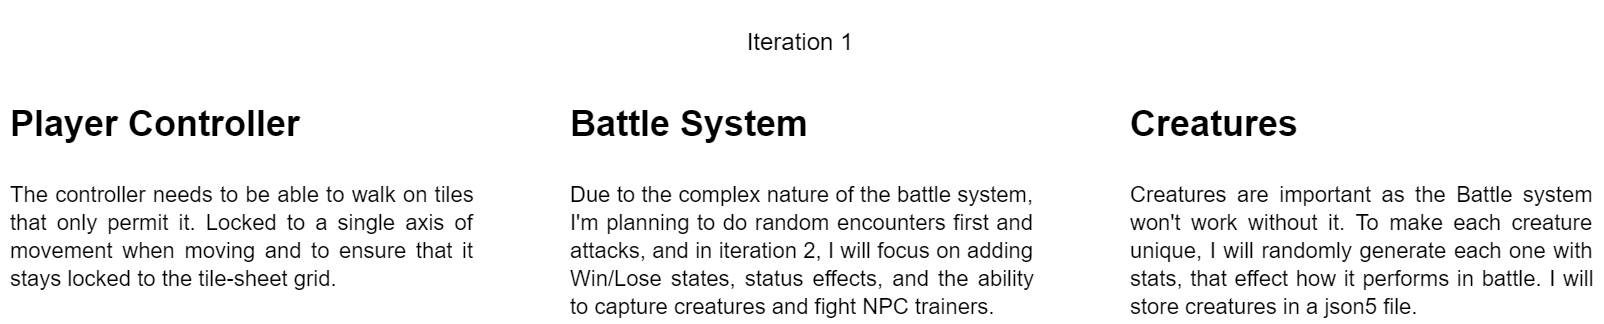
\includegraphics[width=\textwidth]{download (3).png}

\section{Player Controller}
\subsection{Player Movement}
The player will be controlled by a D-Pad, that is featured on the bottom left hand of the screen. The movement is locked to one axis at a time, this is due to the grid based system in place, and instead of it being a technical limitations, its more of staying faithful to the inspiration. When the player moves, it uses a variable, lets call this variable 'move\_offset' and another 'move\_direction', the direction is set to 0 for north, 1 for east, etc. move\_offset is set to 64. Every frame if `move\_offset` is greater than 0, it subtracts 4 and then adds 4, to the player position using the correct offset. This allows the player to stay bound to the grid. The collision works by checking the next tile and the current tile the player is on, first it checks the\begin{wrapfigure}[10]{r,4}{0.5\textwidth}
\begin{center}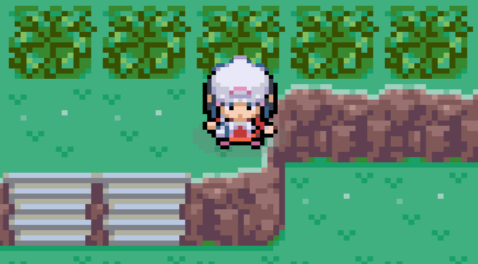
\includegraphics[width=0.5\textwidth,trim ]{Capture.PNG}\end{center}\end{wrapfigure} tile you're trying to move to, and if its possible, it then checks your current tile to see if that tile has one way collision. One way collision is cliff faces for example. You want the player to be able to stand on it, but not walk off it. For example this image to the right, shows a tile that you should be able to walk on but not move on from a certain direction. Special tiles like this are defined in the player controller.


\subsection{Player Sprite}
The player uses move\_direction to show the correct facing sprite, while if move\_offset is greater than 0, it will loop though the correct frames of the movement animation. The tall grass was originally two sprites, the top half and the bottom half, this allowed the player to appear to be standing in the grass, and not just on top of it. However this caused grass draw calls to double, and due to the game being a mobile game I needed to think of a better solution, because 20x20 grass tiles was 800 draw calls. Even though the tile sheet only rendered parts it needed too, and cached many areas, the overlapping tiles required the tile sheet to redraw. If the player moves in and out of a grass tile. To overcome this problem the tile sheet is rendered as a static image( apart from water layers they render each frame of the tile sheet and then loop the rendered image instead of each tile separate ). Now the player appears on top the grass, but we can do a draw in the postdraw loop to draw the lower half of the grass.

But first we need to get the active tile this is calculated by using the following formula. 
$$CurrentTile =((\lfloor\frac{y}{64}\rfloor + 1)\times L) +(\lfloor\frac{x}{64}\rfloor + 1)$$
X and Y is the Player position vector, while L is the amount of tiles in each row. This is done to draw a sprite over the player, if they are currently over tall grass. This allows the game to give an illusion of the player being in the grass.
\begin{figure}[h]
\caption{Notice how when the player starts leaving the tile the grass disappears.}
\centering

\includegraphics[width=1\textwidth]{grass_walk.png}
\end{figure}

\section{Tile-sheet} 
For the tilesheet, I ended up using a framework called gl-tiled, which is easily found on Github(https://github.com/englercj/gl-tiled), It's also perfect as its licence is a MIT License, meaning in the future this project can still benefit from using gl-tiled unlike the other assets used.

\newpage\section{Creature Class} 
The creature class is each instance of a creature, so the base of it. It has multiple values.

\begin{itemize}
\item ARRAY MoveSet -- Stores 4 possible moves that the Creature can use in battle.
\item ARRAY IV -- Randomly generated binary values to determine each one of its stats(HP, Attack,  Defence, Speed, Sp Attack and Sp Defence)
\item ARRAY EV -- Similar to IV apart when defeating a random creature a random stat is chosen to increase allow creatures to get stronger though experience. 
\item STRING Species -- Refers to what species of creature it is.
\item BOOL Gender -- This value is ignored if the creature can only be either female or male or gender-less, if not if the value is true it resembles Male, and false resembles Female which affects certain move types and allows for breeding. 
\item ARRAY Pattern -- This is used by wild and NPC battle creatures to allow for pre-defined move rotations.
\item BOOL Shiny  -- If true give the creature 7\% more health and then set the HUE of the sprite to the Creature Hue.
\item UInt(9) Hp -- The current HP of the Creature.
\end{itemize}

On top of this the class has multiple methods these are;
\begin{itemize}
\item GetData() -- Returns the species array of the base data. See (Section: § Creatures)
\item GetMaxHP() -- Uses the following formula to return the max HP of a creature. $$3+ BaseHP +IV + \frac{EV}{3} \times Level / 80 +Level+11$$
\item Damage(dmgAmt, MoveType, AttackingCreature) -- Uses multiple formulas to determine the strength of the damage the creature takes.  It first takes the current creatures defence (Df) and the attacking creatures attack power(Ap).
$$\frac{\frac{Df}{Ap} \times (\frac{3 *AttackingCreatureLevel}{4} + 4)}{60} + 3
$$ It then sets a variable called 'MoveEffectivenesss' to 1, and it compares both types of the creature to the attacking creature and multiples the multiplier with 'MoveEffectivenesss', the last multiplier is then 1.25 if the attacking creature is using a move that is the same type of the creature using the move, like a fire move from a fire creature.
\end{itemize}

		



\section{Species}
As stated in the above section each creature belongs to a species, the species are stored within a JSON file, which stores details about them.
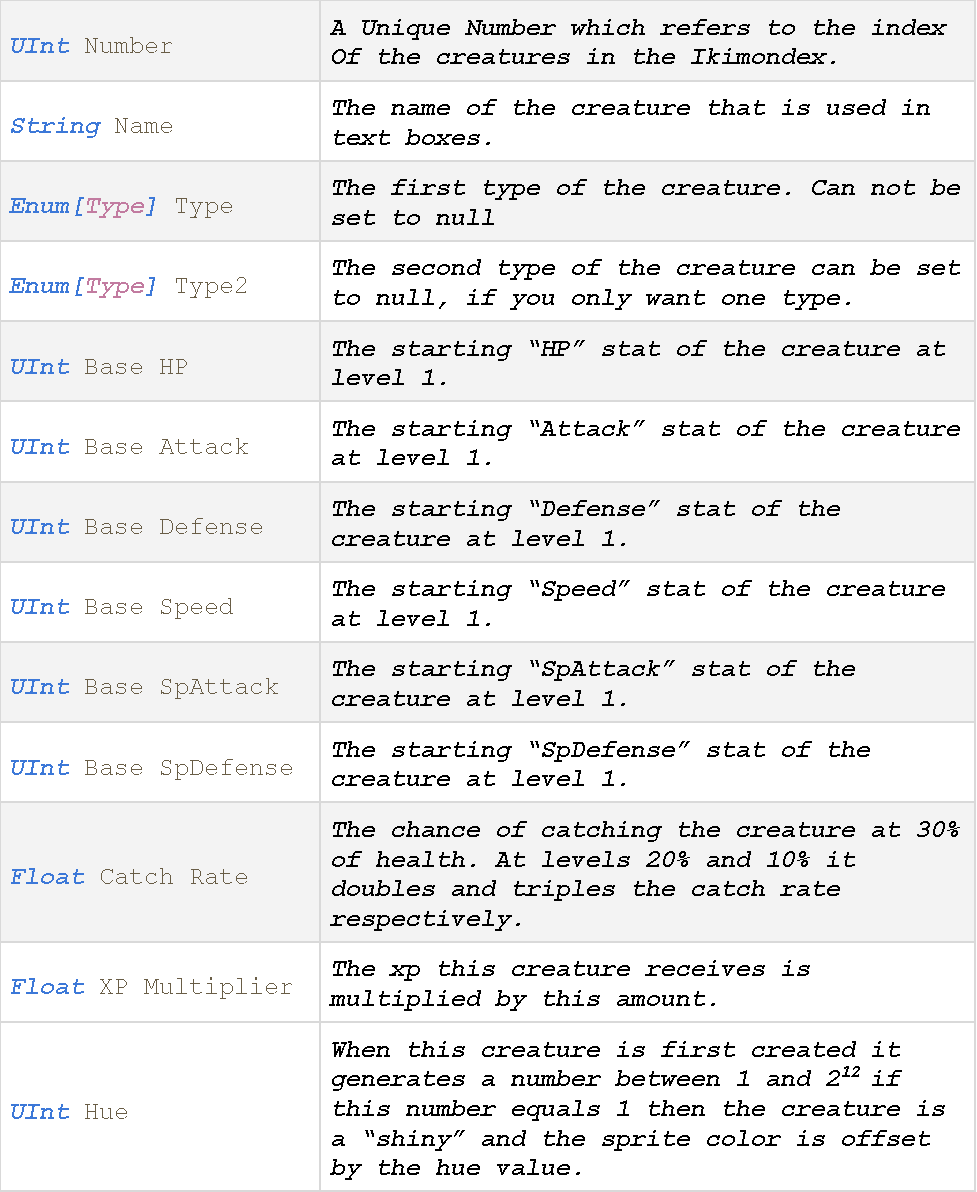
\includegraphics[scale=0.76]{Class.pdf}\newpage
After populating 10 creatures by hand taken roughly an hour to do, I decided to make a spreadsheet. Then I wrote a script to export the spreadsheet to JSON in the proper formatting I needed for the game. Below is an example of the spreadsheet...\\

\begin{adjustwidth}{-127pt}{100pt}
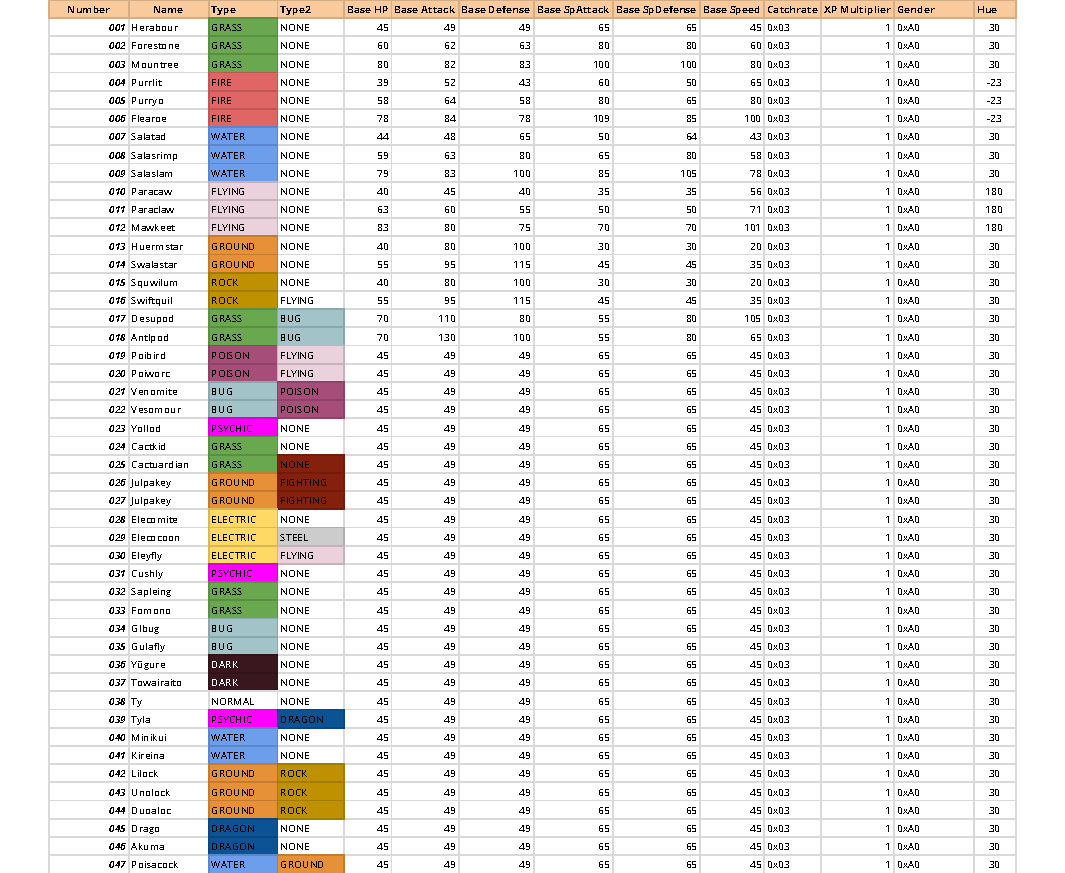
\includegraphics[scale=1.2]{pdfs/Ikimono_sheet.pdf}
\end{adjustwidth}
\nepwage ...and below this is the code to export the spreadsheet to JSON.
\begin{minted}{javascript}
function onOpen() {
    var ss = SpreadsheetApp.getActiveSpreadsheet();
    var menuEntries = [{
            name: "Export as JSON",
            functionName: "exportSheet"
        }
    ];ss.addMenu("Ikimono Tools", menuEntries);}

var COLs = [1, 2, 3, 4, 5, 6, 7, 8, 9, 10, 11, 12, 13, 14]
var HeX = {
    5: true,
    6: true,
    7: true,
    8: true,
    9: true,
    10: true,
    11: true,
    12: true
}

function exportSheet() {
    var ui = SpreadsheetApp.getUi();
    let Ikimonos = {};
    var ss = SpreadsheetApp.getActiveSpreadsheet();
    var sheet = ss.getSheets()[0];
    var range = sheet.getRange("A1:Z100");
    for (let step = 2; step < 100; step++) {
        if (range.getCell(step, 2).getValue() == "") break;
        let Ikimono = {};
        COLs.forEach(function(n) {
            var vv = range.getCell(step, n).getValue();
            if (HeX[n])
                vv = Number(vv)
            Ikimono[range.getCell(1, n).getValue()] = vv;
        })
        Ikimonos[range.getCell(step, 2).getValue()] = Ikimono;
    }

    ui.alert(JSON5.stringify(Ikimonos))

}
\end{minted}

\newpage
\section{Battle}
There are three stages of the battle these are;
\subsection{Generation}
Within this stage, the game generates the creature you're going to encounter, or prepare for an NPC encounter, during this stage the Battle entity is created, and then is populated with the encounter type, if it's a wild creature it will then randomly generate stats, level, its shiny type, gender, etc. It will then start the tweening animation and then transition to the combat. 
\subsection{Combat}
In combat, there is a simple flow in which the combat progresses. The diagram below shows this. The game checks death every-time damage is dealt, when the creature is dead it progress to the end state.
\begin{center}
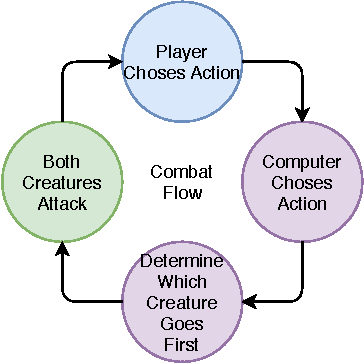
\includegraphics[scale=1.2]{pdfs/combatflow.pdf}
\end{center}

\subsection{End}
If you are the one that died, you're creatures are healed and you are teleported to the nearest Creature Health Centre. If you win, then your creatures in your party are awarded experience and the creature that contributed the most gets an increase in power. It then returns you to the overworld.
\bibliographystyle{plain}
\bibliography{references}
\end{document}
